%----------------------------------------------------------------------------------------
%	PACKAGES AND OTHER DOCUMENT CONFIGURATIONS
%----------------------------------------------------------------------------------------
\documentclass[a4paper]{report}


\usepackage[sc]{mathpazo}
\usepackage[T1]{fontenc}
\usepackage[utf8]{inputenc}
\usepackage[english  ]{babel}
\linespread{1.05}
\usepackage{microtype}
\usepackage{xspace}

\usepackage[hang, small,labelfont=bf,up,textfont=it,up]{caption}
\usepackage[top=4cm, bottom=4cm, left=4cm, right=4cm]{geometry} 
\usepackage{booktabs}
\usepackage{float} 
\usepackage{hyperref}

\usepackage{graphicx}
\usepackage{listings}

%% Usefull for \FloatBarrier
\usepackage{placeins}

\usepackage{lettrine}
\usepackage{paralist}
\usepackage{setspace}
\usepackage{graphicx}

\usepackage{abstract}
\renewcommand{\abstractnamefont}{\normalfont\bfseries}
\renewcommand{\abstracttextfont}{\normalfont\small\itshape}

\usepackage{color}
\usepackage{xcolor}
\usepackage{titlesec}
\usepackage{inconsolata}
%% \renewcommand\thesection{\Roman{section}}
%% \renewcommand\thesubsection{\Roman{subsection}}
% \titleformat{\chapter}[hang]{\bf\huge}{}{2pc}{} 
% \titleformat{\section}[block]{\Large\vspace{0.5cm}}{}{1em}{}
% \titleformat{\subsection}[block]{\large\vspace{0.3cm}}{}{1em}{}

\setcounter{tocdepth}{2}

\newcommand{\ds}{\emph{DataStax\xspace}}
\newcommand{\djd}{\emph{DataStax Java Driver\xspace}}
\newcommand{\ca}{\emph{Apache Cassandra\xspace}}
\newcommand{\px}{\emph{Paxos\xspace}}
\newcommand{\jd}{\emph{Java driver\xspace}}
\newcommand{\cdt}{\emph{Cassandra Detection Tool\xspace}}
\newcommand{\dseg}{\emph{DSE Graph\xspace}}
\newcommand{\om}{\emph{Object Mapper\xspace}}
\newcommand{\sr}{\emph{speculative retries\xspace}}


\lstset{
         basicstyle=\footnotesize\ttfamily, % Standardschrift
         numbers=left,               % Ort der Zeilennummern
         numberstyle=\tiny,          % Stil der Zeilennummern
         stepnumber=2,               % Abstand zwischen den Zeilennummern
         numbersep=5pt,              % Abstand der Nummern zum Text
         tabsize=2,                  % Groesse von Tabs
         extendedchars=true,         %
         breaklines=true,            % Zeilen werden Umgebrochen
            frame=b,         
 %        keywordstyle=[1]\textbf,    % Stil der Keywords
 %        keywordstyle=[2]\textbf,    %
 %        keywordstyle=[3]\textbf,    %
 %        keywordstyle=[4]\textbf,   \sqrt{\sqrt{}} %
         stringstyle=\color{white}\ttfamily, % Farbe der String
         showspaces=false,           % Leerzeichen anzeigen ?
         showtabs=false,             % Tabs anzeigen ?
         xleftmargin=17pt,
         framexleftmargin=17pt,
         framexrightmargin=5pt,
         framexbottommargin=4pt,
         %backgroundcolor=\color{lightgray},
         showstringspaces=false      % Leerzeichen in Strings anzeigen ?        
 }
 \lstloadlanguages{
         %[Visual]Basic
         %Pascal
         %C
         %C++
         %XML
         %HTML
         %Java
         SQL
 }

\DeclareCaptionFont{white}{\color{white}}
\DeclareCaptionFormat{listing}{\colorbox{gray}{\parbox{\textwidth}{#1#2#3}}}
\captionsetup[lstlisting]{format=listing,labelfont=white,textfont=white}

\definecolor{javared}{rgb}{0.6,0,0} % for strings
\definecolor{javagreen}{rgb}{0.25,0.5,0.35} % comments
\definecolor{javapurple}{rgb}{0.5,0,0.35} % keywords
\definecolor{javadocblue}{rgb}{0.25,0.35,0.75} % javadoc
\definecolor{pgrey}{rgb}{0.46,0.45,0.48}

\lstdefinestyle{Java}{language=Java,
basicstyle=\ttfamily,
keywordstyle=\color{javapurple}\bfseries,
stringstyle=\color{javared},
commentstyle=\color{javagreen},
morecomment=[s][\color{javadocblue}]{/**}{*/},
numbers=left,
numberstyle=\tiny\color{black},
stepnumber=1,
numbersep=7pt,
tabsize=4,
showspaces=false,
showstringspaces=false,
moredelim=[is][\textcolor{pgrey}]{`}{`}
}


%%%%%%%%%%%%%DOCUMENT%%%%%%%%%%%%%%%

\begin{document}

\begin{titlepage}

\newcommand{\HRule}{\rule{\linewidth}{0.5mm}} % Defines a new command for the horizontal lines, change thickness here

\center % Center everything on the page
 
%----------------------------------------------------------------------------------------
%	HEADING SECTIONS
%----------------------------------------------------------------------------------------

\textsc{\LARGE University Pierre et Marie Curie}\\[1.5cm] % Name of your university/college
\textsc{\Large Internship Final Report}\\[0.5cm] % Major heading such as course name
\textsc{\large Master's degree}\\[0.5cm] % Minor heading such as course title

%----------------------------------------------------------------------------------------
%	TITLE SECTION
%----------------------------------------------------------------------------------------

\HRule \\[0.4cm]
{ \huge \bfseries Drivers and Tools at DataStax}\\[0.4cm] % Title of your document
\HRule \\[1.5cm]
 
%----------------------------------------------------------------------------------------
%	AUTHOR SECTION
%----------------------------------------------------------------------------------------

\begin{minipage}{0.4\textwidth}
\begin{flushleft} \large
\emph{Author:}\\
Kevin \textsc{Gallardo} % Your name
\end{flushleft}
\end{minipage}
~
\begin{minipage}{0.4\textwidth}
\begin{flushright} \large
\emph{Supervisors :} \\
University : Sebastien \textsc{Monnet} \\
Company : Shannon \textsc{Dennis} % Supervisor's Name
\end{flushright}
\end{minipage}\\[4cm]

%----------------------------------------------------------------------------------------
%	DATE SECTION
%----------------------------------------------------------------------------------------

{\large \today}\\[3cm] % Date, change the \today to a set date if you want to be precise


\vfill % Fill the rest of the page with whitespace

\end{titlepage}


%%%%%%%%%%%%%%%%%%%%CONTENT%%%%%%%%%%%%%%%


\chapter{Introduction}

\pagestyle{plain}
\lettrine[nindent=0em,lines=3]{T} his inter-report describes the content of this internship made at \ds{}, UK, London. The internship was supervised by Shannon Dennis (Senior Director Engineer) and Olivier Michallat (Software Engineer) on the \ds{} side, by Sebastien Monnet (Associate Professor) and Julien Sopena (Associate Professor) on the University side.\\
\subsection{Summary}
I've been joining the Drivers and Tools Developers Team. In this report I will first make a description of \ca{} including some additional research work on software technologies used by \ca{}. Then, I will present the first topic I've been working on, the \djd{} and enumerate the tasks I've been assigned to. I will then describe the second topic of the internship, \cdt{}. The following part will explain the last big topic of this internship, which is the DSE Graph integration in the \djd{}. I will finally conclude by explaining some miscellaneous additional work related to the 3 big topics I've been working on, and conclude.

\chapter{Apache Cassandra}
\lettrine[nindent=0em,lines=3]{A} pache Cassandra is a distributed No-SQL database created by \emph{Facebook} providing high availability and scalability, developed to handle heavy workload produced by their large amount of users and data. \ca{} has a master/slave-free architecture which allows it to provide linear scalability and helps instant recovery on hardware and software failures.\\
The purpose in the following is not to make an entire technical description of \ca{} since on the one hand, the internship doesn't involve me on the internal development of \ca{}. On the other hand, understanding all concepts of \ca{} is important to be able to handle correctly the interaction with an \ca{} cluster and thus, be as efficient as possible in the development of the \djd{}.

\section{General Concept}
With \ca{}, each node on a cluster of machines is responsible of a part of the data. Thus, a set of data is represented by a Partition Key, and this Partition Key indicates on which node it will be stored, since at each node is attributed the responsibility of a range of Partition Keys. The data can (and is supposed to) be replicated among other nodes with a coefficient of replication that involves different policies of consistency and load balancing. All \ca{} nodes will then refer to these policies to manage data among all other nodes.\\
Wrtiting on a replicated data introduce consistency challenges and is handled in \ca{} by broadcasting the \verb;write; operations on all replicas and then waiting on a quorum of replicas to confirm that changes have been applied. A default setting on an \ca{} node is to set this quorum's size to \emph{N/2} (N is the number of nodes owning a replica of the data). \verb;Reads; on replicated data can be configured according to the client's requirements. Each Cassandra node is aware of all the other nodes, and each node is responsible of the replication of the data in his range of Partition Keys.

\section{Advanced Description}
The following section will describe more precisely some of the key features that allows \ca{} to achieve its high availability and scalability characteristics. We will also make some comparison with other database systems that have different behaviors regarding these characteristics.
\subsection{Transactions}
\ca{} version 2.0 introduced a system to handle distributed transactions which, for instance allows clients using CQL operations like :
\vspace{0.7cm}
\begin{lstlisting}[label=cql-ex-1, caption=CQL Update Example, language=SQL]
UPDATE ExampleTable
SET variable = NEW_VAL
IF variable = OLD_VAL;
\end{lstlisting}
\vspace{0.7cm}
This \emph{IF} condition may not be a big constraint when developing a relational database, but with a fully distributed database, this precondition causes several complications : 
\begin{itemize}
	\item How to achieve linearizability and consistency with distributed transactions ? Use Consensus.
	\item How to keep an acceptable throughput with a Consensus algorithm ? \px{}\cite{Lamport1}.
\end{itemize}
{\bfseries But}, building these types of transactions involved the need to add some extra-phases to the original \px{} algorithm. Here we won't recall \px{}'s proofs that define the Consensus guaranties when a majority of nodes responds positively in the \emph{Accept} phase. But original \px{} algorithm allows to agree on one value that won't be changed, besides that, what we want to do in \ca{} is to achieve linearizibility on a suite of operations (or we can say 'values'). Nodes would then be sure of the consistency of the data since every node would have executed operations on its replica in the same order. \\
To do so, a node must find a way to 'restart' the algorithm in order to make a new decision on another value and chain the algorithm executions. First way to do that would be to build a distributed edit log file based on successive Consensuses made with \px{} (a brief review of \emph{Google}'s solution to do that later). To chain \px{} execution in \ca{} the idea has been to add an extra phase to the algorithm called \emph{commit} phase which simply sends \emph{commit} messages to all nodes to notify them the end of the algorithm.\\
Another point about using \px{} algorithm in our context is that our need is to execute a \emph{compare-and-set-like} operation, whereas \px{} algorithm allows to only \emph{set} a value without making the comparison. \\
Making this possible implied adding another extra-phase to the original \px{} algorithm, which is, after receiving a majority of responses from the \emph{prepare} phase. The newly decided coordinator will send a request to all nodes to get their local value of the replica. If the expected value match, the node proceeds to the following of the algorithm (\emph{accept}), if not, the algorithm stops and the value is not updated.
With these solutions, \ca{} simply implements \emph{compare-and-set} distributed operations on multiple variables sequentially with the guaranties of the \px{} algorithm. With the cost of the overhead produced by the 2 extra-phases.

\subsubsection{\emph{Google}'s distributed edit log file}
\emph{Google}'s approach to build a distributed fault-tolerant database based on \px{} was described in their paper \emph{Paxos Made Live}. It actually explains that even if \px{} algorithm could be easily described in one page of algorithmic instructions, engineering a production-ready software based on it, is not so simple.\\
Indeed, to be fault-tolerant an application has to rely on the hypothesis that a machine doesn't have unlimited memory, and that it can suffer of hard disk failures. Also, the implementation has to be adaptable to different hardware infrastructures since real systems are rarely specified precisely.\\
The approach taken here was to build a \emph{fault-tolerant} log file that will be describe the operations to be applied on a replica of data. All the replicas hosts would then agree with \px{}'s Consensus on the content of this log file and each one would keep locally a version of it. Building a file log of sequential operations implies to chain \px{} executions, which are called \emph{instances} (the same idea described earlier for \ca{}).\\
In order to increase throughput and performance of the \emph{instances}, two additional concepts came up in the paper : 
\begin{itemize}
	\item When a coordinator sends data in an \emph{Accept} message, it can concern not only one variable, and update multiple set of variables. So when the \emph{Accept} message is acknowledged by a majority of nodes, all the values will be modified at the same time.
	\item To avoid as much \emph{Propose} messages overhead as possible, the algorithm could state that a coordinator, once it has passed the \emph{Accept} phase with his value on a previous instance, can stay \emph{elected} for certain period of time. And thus, it can chain \emph{Accept} phases for as long as he is coordinator. He is then called \emph{master}. After that, when a node starts a new instance of \px{} algorithm, it first tries to grant a lease from the coordinator (\emph{master}) of the last instance and sets it as his coordinator for this new instance.
\end{itemize}
\emph{Master} leases doesn't corrupt the \px{} algorithm since a \emph{master} is elected it can fail, and after a certain period of time (\emph{heartbeats}), a new instance will be run and will elect a new \emph{master}.\\
Besides that, \emph{master leases} improve performance with the fact that when a \emph{master} is elected by a majority of replicas, the \emph{compare} of a \emph{compare-and-set} operation on a \emph{master} can be done locally since once it knows that it has been elected, the \emph{master} knows no other node is going to acknowledge \emph{Propose} messages from another coordinator. Each time a \px{} instance is ran, replicas \emph{grant} a lease from the \emph{master} of the previous instance. For \emph{Google}, this implementation of \px{} was used as backend of \emph{Chubby}, a \emph{fault-tolerant master-slave} distributed locking system which during its computation stores \emph{Chubby} lock files in a distributed database with replication, and that was then, using this implementation of \px{}. This way, \emph{Chubby masters} and \emph{Paxos masters} could be correlated to improve throughput of the application.\\
Since the log file concerns actions to be applied on a certain data structure, the data structure's history has to be saved, so as for the log file, in case of when a replica fails and has to recover. To handle limited memory restrictions, persistent state's history has been achieved by making \emph{snapshots}. With a proper \emph{snapshot} algorithm the data could be saved in a period of time related to the memory capacity and the \\
log file can also be truncated since it only needs to contain the operations executed since the last \emph{snapshot}.\\
Implementing these concepts and other technical details allowed to build distributed fault tolerant database relying on \px{}.

\subsection{\ca{} local persistence} % (fold)
\label{sub:ca_local_persitency}

To achieve local persistence of writes on data in the most efficient way, \ca{} rely on some principles that helps acquiring better performance and safety.\\
Each write operation involves a new entry in a local commit file. The write in this file is persisted and it is assumed in \emph{Facebook}'s paper on \emph{Cassandra} that this commit file is stored on a dedicated hard disk used only for this purpose, to maximize throughput in regard of the sequential constraints of this one.\\
To optimize response time on a \emph{read} request, \ca{} first does a lookup in the in-memory data structure of most recent data, and if not present, do a lookup on persistent storage. Data is stored in many files on a disk, (ordered from newest to oldest) each part of the data represented by a key. To prevent browsing files that do not contain the needed key, each file owns an index which describes all the keys the file is composed of. This index is called \emph{bloom filter}.

% subsection ca_local_persitency (end)

\subsection{Gossip membership protocol and possible ATTACKS} % (fold)
\label{sub:gossip_membership_protocol_and_potential_weaknesses}

With \ca{}, since the data is distributed and replicated, each node maintains locally the situation it is aware of each other node in the \emph{ring} (the \emph{ring} represents the nodes organized according the distribution of the tokens). \\
To maintain a coherent distribution of the tokens, in case of when a node fails, a membership protocol called \emph{Gossip protocol} runs regularly to keep the ring coherent. In short, this this protocol consists of : an \emph{initiator} node starting a \emph{gossip} round by sending a \emph{receiver} node his current view of all the nodes. The \emph{receiver} updates his view according to the initiator's view (assuming that there's a additional technical process that can insure that a view is more recent than another). And if the view also needs to be updated on the \emph{initiator}, the \emph{receiver} sends the updates in an \emph{ack} message. The \emph{initiator} then updates his views and acknowledges them to the \emph{receiver}.\\
After explaining that this protocol brings a great benefit to the consistency of the system, we will see that some experiences proved that in some cases it can also become a weakness...\\
This\cite{Aniello13} paper explains the vulnerabilities to such a protocol, stating that, in the \emph{gossip} protocol, there is no concern about the about what could happen if the information in these \emph{gossip} messages are false, corrupted. With this statement, we can imagine 2 types of of attacks involving a byzantine node that's purpose is to send wrong information among the network.\\
A first \emph{attack} would be to make some nodes (even maybe all) believe that a node is \emph{down} while he is not. Sending a message to a \emph{receiver} node, falsely up-to-date, saying that a node is \emph{down} can lead the \emph{receiver} node to update his view with a wrong information. The second \emph{attack} is the opposite of the first one, a byzantine node waits for a node to fail, and while the node is failed, the byzantine one sends \emph{gossip} messages to every other saying that for it (the last updated view) the node is still up.\\
This kind of \emph{attacks} can have a big impact on the performance of the database when there's big loads of data to handle. \\
It could in the first case, contradict load balancing policies by lowering the usage of the \emph{faked} node, in the second case, involve a great number of lost requests. The paper reports a percentage of up to ~83\% of lost requests when disseminating up to 75\% byzantine nodes in the network, using the \emph{ALL} consistency level. It also describes a \emph{relatively low} performance impact solution to the excess of trust in the \emph{gossip} protocol. It consists in adding an encryption layer to the protocol, allowing to insure that information provided is not from a byzantine node. A little bit like Byzantine \px{}\cite{Martin}, with the cost of encryption.

% subsection gossip_membership_protocol_and_potential_weaknesses (end)

\chapter{Java Driver for Apache Cassandra}
\lettrine[nindent=0em,lines=3]{T} he first and main topic of this internship have been to contribute to the open-source project \djd{}. Thus, I will describe how the \djd{} represents more than a simple software that sends packets to a server, by explaining some of its most important and useful characteristics. I will after expose some notable features I've been helping adding in the driver, then present the features I have been working on by myself.
\section{Introduction}
The \djd{} is a high level library that handle interaction with a \ca{} database. The \djd{}'s main goal is to successfully establish connection to a node, send requests and receive results. It is closely tied to the \emph{Cassandra Query Language} and communicates with \ca{} using a communication protocol named \emph{Native Protocol}.

\section{Basic concepts}

\subsection{Connection}
The first step, to successfully achieve communication with a \ca{} database is to be able to successfully connect to it through the network. With the \djd{}, it is possible to connect to any of all the nodes in the Cassandra cluster by providing at least one IP address of one node.\\
The main representation of the connection to a \ca{} cluster is exposed through a \emph{Cluster} object. To optimize latency, throughput and scalability (more on that later), the driver will then gather a lot of information from the node it is connected to. The first node connected, becomes what we call the \emph{Control connection}. After connecting to the first node, the driver will execute several additional tasks :
\begin{itemize}
   \item Connect to all other known up nodes in the cluster.
   \item Collect cluster metadata.
   \item Collect schema metadata.
\end{itemize}

After these tasks successfully executed, a \emph{Session} object is returned to the client. This \emph{Session} object is the object from which the client will be able to send, prepare, and bind \emph{CQL} statements.

\subsection{CQL}
The \emph{CQL} query language is a database query language specific to \ca{}. Its purpose is to fit the most possible to the existing universal \emph{SQL} query language, and in the same time provide \ca{} specific syntax. \emph{CQL} is then designed to provide options and tools to handle distributed datasets, with the possibility to manage consistency levels, replication factors, data partitioning, node management, and so on. \emph{CQL} statements are sent by the driver to a \ca{} cluster through the \emph{Native protocol}.

\subsection{Native protocol}
The \emph{Native protocol} is a network applicative protocol built on top of \emph{TCP}. It has been designed to be fully asynchronous, hence, on the driver side it allows to accumulate queries on a single connection in an asynchronous manner. Indeed, each request on a connection gets assigned to a request identifier, named stream id, created in a thread-safe way on the client side. Multiple requests can be sent asynchronously and concurrently through the connection, each response coming back will be assigned to the stream id it has been issued from. The driver also adds a client-side timestamp on each request, to insure order of requests when needed by the user.
\emph{Native protocol} also allows security functionalities like server-side authentication and SSL encryption.\\
Most of the work accomplished by the \djd{} is to encode and decode data sent and received through the \emph{Native Protocol}.

\subsection{Processing responses}
The \emph{Native protocol} being fully asynchronous, a client has the possibility the process the results of its queries either synchronously or asynchronously. Internally, everything is handled asynchronously, every request implies the creation of a \emph{Future} object from the Java's \emph{Future} library. On these \emph{Future} objects we can define callbacks to fill the data when a connection notifies that the data has arrived through the connection. Since internal processing in the driver is asynchronous, most part of the code is thread-safe.

\subsection{Metadata}
Aside from sending statements, and processing results, the \djd{} exposes a complete description of the cluster, schemas, tables, indexes, partitions, through the \emph{Metadatas}. This metadata is computed at the \emph{Cluster}'s initialization and is maintained up-to-date all along the \emph{Cluster} object life span. Having this metadata improves the driver knowledge of the current status of the system, and allows the driver to adapt it's behavior according to it. The metadata is also exposed to clients through API specific objects.



\section{Advanced Features}
In this part I will try to explain some more advanced features that contribute in making the \djd{} more powerful, scalable, tunable, and probably jusifies the 70.000+ public downloads of the software each month. I will present these features in details because we'll see later that some of my assignments for the internship were to maintain, or improve those features, and acquiring a strong understanding of these notions have also been the first step of the internship.

\subsection{Connection Pooling}
As stated before, at cluster initialization, the driver establishes connection to the first IP address that has been specified, and this node becomes for the driver, the \emph{Control connection}. In addition to that, the driver will also establish a connection to all the other nodes in the cluster. This is made for multiple purposes. First, in case of a clear failure on a node, which doesn't respond in time (timeout), or returns an internal exception, so the driver still has a way to process the request for the client. Remember that \ca{}'s architecture is Master-less, which means every node is able to handle every request, the nodes are aware of the data repartition (Token routing) and replication. The second advantage of connecting to all nodes is load balancing. Indeed, to handle heavy loads needed for some applications, the driver is able to distribute the requests to all nodes equally, so that one node connected doesn't get overloaded (more information in the \emph{Policies} section).\\
But that's not all, to achieve even better throughput the driver establishes pools of connections for each host. This is needed mainly because requests can take a viariable amount of time to be executed on the server side, and since everything is asynchronous, the protocol accepts adding pending requests on a same connection (thanks to stream ids). But it has its limits, the \emph{Native protocol} version 2 can only handle a maximum of 128 simultaneous requests on a same connection. This limit can quickly transform into a bottleneck, that prevents achieving high throughput. That is why the driver has pools of multiple connections for each node.\\
Unfortunately achieving high throughput comes with the price of having to tune and maintain the connection pools. Thanks to the highly tunable nature of the driver, users are able to define rules to dynamically resize connection pools according to the current load. Indeed when the load becomes more consequent, the driver automatically increases the number of connections in the pools. We can detect that the load becomes heavier because the driver maintains a number of pending requests per each connection. Hence, the decision to open a new connection is made when all existing, except one, connections in the pools have the maximum allowed pending requests, and when the number of pending requests on the last connection becomes higher than a defined \emph{threshold}.\\
The driver provides the option to set the original number of connection per pool, the maximum number of connections to create, and set the \emph{threshold} to use for connection creation, and also set the \emph{threshold} indicating whether to close a un-needed connection.\\
With fine tuning of these parameters, our experiments prove that the driver is able to issue comfortably a total of 100k requests/node.\\
In more recent versions of \ca{}, the \emph{Native protocol} have been updated and is now able to support 32768 requests on each connection. This greatly helps improving the usage of a connection pool, unfortunately experiments still show a bottleneck in using a limited number of connections in pools, more on that later, in the \emph{Netty} section.

\subsection{Policies}
The Java driver is highly tunable, and some of its most important settings are defined with policies. A policy is a Java object defined by the user, implementing an \emph{Interface} of the driver, and whose methods will be injected used in the driver's code. The user can specify the policies during the cluster's creation.

\subsubsection{Load Balancing Policy}
The driver provides a set of pre-configured and highly tested load balancing policies. However, a user can injects its own. The load balancing policy is the class defining the \emph{query plan}. The \emph{query plan} is the object which defines what will be the host chosen to send each query, it's a Java \emph{Iterator} which will return a host each time the driver needs to send a request. This setting is important in order to distribute the load on as much nodes as possible and thus, avoid bottlenecks and improve throughput.\\
For example, the most common and meaningful balancing policies to use, for normal use-cases is the \emph{TokenAwarePolicy} with a \emph{DCAwareRoundRobinPolicy} fallback option. 
It is set constructing the following object a cluster's creation :
\begin{lstlisting}[label=lbp-ex-1, caption=Creation of the cluster, language=Java]
Cluster.builder()
   .withLoadBalancingPolicy(new TokenAwarePolicy(new DCAwareRoundRobinPolicy, true));
\end{lstlisting}
This setting allows to send statements to directly to hosts having a local replica of the data according to the routing key of the statement (that's the goal of the \emph{TokenAwarePolicy}) and if no local replica was found, send the statement in a round-robin fashion, to hosts from the same DataCenter (the role of the \emph{DCAwareRoundRobinPolicy}).\\
Other useful Load balancing implementation are provided from the driver such as \emph{WhiteListPolicy}, or \emph{LatencyAwarePolicy}. But users can still implement their own policy and inject it in the driver. By default the driver uses a \emph{RoundRobinPolicy} based on its knowledge of the hosts located in Cassandra's table \emph{system.peers}.

\subsubsection{Retry policy}
The retry policy defines what should be the behavior of the driver in case a query sent to a Cassandra node happens to fail, and the node originally contacted for the request sends back to the driver the error corresponding.\\
Executing a query can fail in two ways : 
\begin{itemize}
   \item The error happens on the driver side. The driver is not able to communicate to the server in the required time, or no host is available anymore, a network failure occurs.
   \item The coordinator (host contacted for the query) is reachable for the driver, and the coordinator receives the query, but an issue internal to the processing on the server-side occurs. This can be a consistency level issue, a network issue between multiple Cassandra nodes, and so on.
\end{itemize}
For the first case, the driver provides an API to tune the socket options. With this, users can set timeouts, buffer sizes, etc.
The second point is handled differently, when a server-side issue occurs, the coordinator will be able to send an error message to the driver. Then, the reaction of the driver according to different kind of errors will be defined by a \emph{RetryPolicy}.
The errors returned can be of 3 types : 
\begin{itemize}
   \item Read timeout
   \item Write timeout
   \item Unavailable host
\end{itemize}
Each of these errors is likely to happen because the consistency level required for the query could not be met (e.g if 3 replicas were required but only 2 responded within the defined server-side timeout). Then, the driver will call the corresponding method in the \emph{RetryPolicy} object it has been constructed with. If the error is a \emph{ReadTimeoutException}, the driver will call \emph{RetryPolicy.onReadTimeoutException()}.\\
As usual, the driver provides highly tested and pre-configured Retry policies. An interesting one is the \emph{DowngradingConsistencyRetryPolicy}. Thanks to this policy, we can define that when a \emph{ReadTimeoutException} happens, the driver will re-send the request, to the same host, with a consistency level reduced by 1 and only once, otherwise a Java exception is thrown.

\subsubsection{Reconnection policy}
A reconnection policy is meant to be used in cases where a connection in a pool gets closed because of a particular error. The reconnection policy mainly helps define the time before the next reconnection attempt gets scheduled. Users can explicitly set this time, or \emph{ConstantReconnectionPolicy} can help define a constant time before reconnection, and \emph{ExponentialReconnectionPolicy} helps define a base delay which will grow exponentially, until a maximum delay is reached, then when the maximum is reached, it will stay constant.

\subsection{Object Mapper}
The \om{} is an additional module of the driver, distributed as a separate Maven artifact. This module provides a simple object mapping that avoids most of the boiler plate of converting CQL results to and from a Java object. It handles basic CRUD operations in Cassandra tables containing UDTs, collections and all native CQL types.\\
The object mapper is configured through annotations. The \om{} can map all native \emph{CQL} types and also collections, user defined types. The following is an example of its usage : 

\begin{lstlisting}[label=om-ex-1, caption=Object Mapper example, style=Java]
`@UDT(keyspace = "ks", name = "address")`
class Address {
    private String street;
    `@Field(name = "zip_code")`
    private int zipCode;
    // ... constructors / getters / setters
}

`@Table(keyspace = "ks", name = "companies",
       readConsistency = "QUORUM",
       writeConsistency = "QUORUM",
       caseSensitiveKeyspace = false,
       caseSensitiveTable = false)`
public static class Company {
    `@PartitionKey`
    `@Column(name = "company_id")`
    private UUID companyId;
    private String name;
    private Map<String, Address> aMap;

    // ... constructors / getters / setters
}
...

/* Application code */
Mapper<Company> mapper = manager.mapper(Company.class);

UUID companyId = ...;

Map<String, Address> map = 
                     new HashMap<String, Address>();
map.put("office1", new Address("street1", 01000));

Company c = 
        new Company(companyId, "GreatestCompany", map);

mapper.save(u); //The mapper persists the object
\end{lstlisting}
The mapper also provides accessors, and has its set of \emph{Option}s for tuning.

\subsection{Query builder}
The query builder is another module of the driver, that comes packaged with the driver core component. As its name states, the query builder helps creating valid \emph{CQL} queries in an object oriented fashion. It handles most of the possibilities offered in the \emph{CQL} syntax.\\
Here's a quick example : 
\begin{lstlisting}[label=qb-ex-1, caption=Query Builder example, style=Java]
QueryBuilder builder = new QueryBuilder(cluster);
Statement select = builder.select().all().from("foo").where(gt("k=1 OR k", 42)).limit(42);
// Result is : "SELECT * FROM foo WHERE \"k=1 OR k\">42 LIMIT 42;"
\end{lstlisting}



\section{Notable new features}
The previously presented features compose the core functionality of the driver. However, since the beginning of this internship, some other interesting features have been added, on some of them I've been helping and contributing.

\subsection{Speculative retries}
\emph{Speculative retries} is a way to improve a query execution in case a host happens to be long to respond, because of a GC pause for example. Where \sr{} acts, is that the driver will automatically, transparently for the user, send the statement to another host in case it responds faster.\\
In case speculative retries are fired, the previously sent statements are canceled on the hosts.\\
\begin{figure}[ht!]
\centering
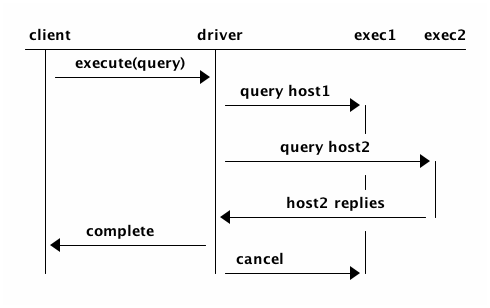
\includegraphics[scale=0.7]{spec_rec.png}
\caption{How speculative retries work \label{overflow}}
\end{figure}
With \sr{} comes the question to know when a statement is idempotent or not. Indeed, in \ca{} a statement is not idempotent when it : 
\begin{itemize}
   \item update a counter\footnote{A counter is a special column type in \ca{} that's optimized and tunable in consistency and cache options on the server side. A counter can only be incremented or decremented by reading the current value and applying a \emph{delta}. Thus, the nature of this type is non-idempotent.} ;
   \item adds an element in a collection like a list ;
   \item uses non idempotent \emph{CQL} functions like \emph{now()}.
\end{itemize}
Hence, since the driver does not parse text \emph{CQL} statements that it sends to the server, a conservative approach has been taken and all statements are considered as non-idempotent by default. Users have to explicitly indicate that the statement is idempotent through a statement \emph{option}. The only moment when the driver can know if a statement is idempotent, is when the query is constructed with the \emph{Query Builder}.\\
\emph{Speculative retries} are configurable on the delay new retries are scheduled. This delay is compatible with another driver component, the \emph{Latency Tracker}.



\chapter{Achieved work}
The main purpose of this internship at DataStax is to contribute to the active development of the open-source \djd{} for \ca{}. This includes aggregating the client's API with new functionalities to fit \ca{} functionalities, internal operation of the driver, improving Query Builder\footnote{Query Builder is a library developed for the Java Driver allowing clients to build query in an Object Oriented way. \textit{Example : Statement statement = QueryBuilder.select().all().from(keyspace, table);}} 
and Object Mapper \footnote{Object Mapper is an Object Relational Mapping tool developed for the Java Driver.} 
functions, resolving reported internal driver's issues and suggestions. I will then, give a brief description of some of the most significant tasks I have been working on since now. I have also been assigned to build a new \ds{}'s tool called \emph{Cassandra Detection Tool} (described later).

\section{Java-Driver}
\subsection{Refactoring Integration Tests Class}
The test architecture for the \djd{} is composed of both unit and integration test. Those test are ran 24/7 for continuous integration by \emph{Jenkins} servers. To simplify building these tests, a big number of integration tests are classes that extend an \emph{all-configured} class which has the responsibility to create the necessary connections and configurations with a test cluster using DataStax's specific tools for automating \ca{} cluster creation.\\
The previous behavior was that inheriting this all-configured implied the need to recreate a new cluster each time. The process was simplified by creating a generic class that initiates a cluster and stays instanciated for all classes inheriting it, adding a thread-safe need for this class. Integration tests suite runs approximately 30\% faster.
\subsection{Manual Paging}
Requests on \ca{} that generate a large amount of data are transfered in network applicative frames called \emph{pages}. These pages are identified by \ca{} and are communicated through the \emph{Native protocol}. The goal of this improvement was to give client the possibility to handle themselves the \emph{paging state} of a request. Thanks to his \emph{paging state} the client start fetching some data from the server, stop processing, and re-send a new request but with the \emph{paging state} information which allows him to continue its processing from where he had stopped. Giving the possibility to the driver to be used in a entirely stateless environment. This task involved studying \emph{Native protocol} and gathering information by manually decoding frames, changing the internal use of the \emph{paging state} in the driver and understanding \ca{}'s usage of the \emph{paging state}.
\subsection{Asynchronous host pools creation} % (fold)
\label{sub:asynchronous_host_pools_creation}

Until now, creating a pool of connection to a \ca{} node was all made sequentially. Moreover, making an authenticated connection on a \ca{} cluster implies a certain overhead due to password verification. Therefore, when the driver has to make sequentially a pool of authenticated connections it could imply too much latency on a cluster with a large number of nodes.\\
The solution was to make the pool creation entirely asynchronous. Thus, all connection pools are made in parallel, and the driver worker only have to wait for all connections to be established. Since we are in a HIGHLY concurrent part of code, lots of issues were produced when adding this feature and needed a big part of refactoring of code. Temporary tests report a improvement 8x the time for the driver to connect to a 40 nodes cluster.

\section{Cassandra Detection Tool}
\emph{Cassandra Detection Tool} is a software I have been asked to contribute to that's main function is to provide to customers all useful \ca{} information we can gather concerning a given a range of IPs. Customers owning a (\emph{very}) large number of clusters among its network sometimes isn't even sure how much nodes are running. \emph{Cassandra Detection Tool} makes then, a clean and concise description of the \ca{} instances. 
A first prototype of the tool has been made by \emph{Martin Van Ryswyk}, our Executive Vice President in Engineering, and my work have been to build a final working solution of the software.\\
It turned out that I changed almost all the code conserving the original conception design. Technically the process was to first, use asynchronous Java sockets to try to establish connection on all of the given IP, all tries made in parallel. Thanks to that the software could establish a list of UP nodes running a \ca{} instance. Moreover, the app use the \djd{} and  the \emph{Java Thrift API}\footnote{Apache Thrift is a network applicative protocol originally used for Cassandra but got replaced by the Native protocol because of performance issues and also because the Java API for Thrift was really hard to use and not well designed. It is still available (but not updated) and Deprecated but I use it here for compatibility with clusters potentially using an old version of Cassandra.}
to connect to running hosts and gather all the node information possible. Information concerns : token map, cluster's hosts, keyspaces and all types of versions. To be more efficient in case of a \emph{big} list of hosts (we can aim for a class B network) to connect to, the application creates a dynamic sized thread pool and then tries to use drivers to gather information. Also, to avoid the need for a thread in the pool (\emph{worker}) to have to, let's say, send gathered information to a main worker that processes all the results and etc... the information was stored in \emph{static} (shared) data structures so it was highly concurrent because a certain number of nodes can be located on the same cluster, and modifying the list of nodes in this \emph{Cluster} object has to be doable concurrently. As a result, the code is thread-safe.\\
It was great to have the opportunity to build this software on my own, and also I'll have the chance to make a video presentation to clients and sales team people on how to use the software (even though I tried to make a GUI as clean as possible).


\chapter{What's next}
For the following of the internship I will continue to contribute to the \jd{} bringing new functionalities and trying to understand more and more of its code in order to be able to handle more easily the development process.






% subsection asynchronous_hosts_pool_creation (end)



\begin{thebibliography}{99}
  \bibitem[1]{Lamport1} Leslie Lamport.
  	\newblock \textit{Paxos Made Simple.}
  	\newblock ACM SIGACT News (Distributed Computing Column), 2001.

  \bibitem[2]{Google1} Tushar Chandra, Robert Griesemer, Joshua Redstone.
  	\newblock \textit{Paxos Made Live - An Engineering Perspective.}
  	\newblock June 20, 2007.

  \bibitem[3]{Aniello13} Leonardo Aniello, Silvia Bonomi, Marta Breno, Roberto Baldoni.
    \newblock \textit{Assessing Data Availability of Cassandra in the Presence
of non-accurate Membership.}
	\newblock University of Rome, Italy, 2013.
  
  \bibitem[4]{Martin} Jean-Philippe Martin, Lorenzo Alvisi.
    \newblock \textit{Fast Byzantine Paxos}.

\end{thebibliography}



\end{document}

















































